\documentclass[11pt, a4paper]{article}

\usepackage{listings}
\usepackage{color}
\usepackage[normalem]{ulem}
\usepackage{graphicx}

\setcounter{section}{-1}

\definecolor{dkgreen}{rgb}{0,0.6,0}
\definecolor{gray}{rgb}{0.5,0.5,0.5}
\definecolor{mauve}{rgb}{0.58,0,0.82}

\lstset{frame=tb,
  language=SQL,
  aboveskip=3mm,
  belowskip=3mm,
  showstringspaces=false,
  columns=flexible,
  basicstyle={\small\ttfamily},
  numbers=none,
  numberstyle=\tiny\color{gray},
  keywordstyle=\color{blue},
  commentstyle=\color{dkgreen},
  stringstyle=\color{mauve},
  breaklines=true,
  breakatwhitespace=true
  tabsize=3
}

\begin{document}
\title{}
\author{Groep A\\ Rapport 1}
\date{19 maart 2014}
\maketitle


\section{Enkele opmerkingen over dit rapport}
We hebben ervoor gekozen om verder te bouwen op het rapport van de vorige keer. Grote delen van de tekst zijn dus dezelfde als een maand geleden. Op die manier behandelt ook dit rapport alle functionaliteit van de website, en is het niet nodig om het vroegere rapport erbij te leggen. Volledig veranderde en nieuwe (sub)secties zijn 'Status', 'Taakverdeling', 'Voorspellingen van gebruikers',  'Extra functionaliteit' en 'Planning'. Licht aangepaste (sub)secties zijn 'Design' (zonder subsecties) en 'Database'.
\section{Status}
Er is heel wat data toegevoegd aan de database; die bevat momenteel honderden teams en duizenden spelers. De database moet uiteraard nog steeds verder groeien. Daarnaast is ook de mogelijkheid om als ingelogde gebruiker voorspellingen uit te brengen toegevoegd. Heel wat bugs zijn gefixt. De site staat ondertussen ook online (www.coachcenter.net), maar na een wissel in servers zijn de meeste pagina's onbereikbaar geworden. Het is dus nog steeds aangewezen de lokale versie te gebruiken. Verder zijn er geen grote features toegevoegd; het project lag na de vorige presentatie een tijdje stil door een combinatie van een aantal plotse andere taken en drukke vakanties van de groepsleden.

\section{Taakverdeling}
\subsection{Stijn}
Verzamelde heel wat meer data, vond nieuwe bronnen voor data. Refactorde grote delen van de code met oog op snelheid, effici\"entie en modulariteit. Betreft het design, is het nu een stuk eenvoudiger om aanpassingen door te voeren (vb. extra data van een speler parsen).
\subsection{Kristof}
Regelde een server om onze website online te krijgen, en ging aan het werk om de website online ook effectief aan de praat te krijgen. Fixte ook verschillende bugs.
\subsection{Tom}
Werkte aan de implementatie van het voorspellingsalgoritme.
\subsection{Jakob}
Werkte aan de interface om gebruikers voorspellingen uit te laten voeren.
\subsection{Ruben}
Zorgde voor specifieke bugfixes.

\section{Design}
De meesten van ons groepje hadden totaal geen ervaring met het bouwen van websites. In het begin van het project zijn de meesten dus begonnen met het doornemen van allerlei tutorials. Dit nam redelijk wat tijd in beslag, waardoor het eigenlijke project met wat vertraging begon. In eerste geval werkten we aan de backend van de website: opstellen van databaseschema, bouwen van loginsysteem, ... We waren eerst van plan om onze data te verkrijgen via de OpenFooty API. Ongeveer een week na het versturen van onze API key request begonnen we te vrezen dat we deze niet meer gingen krijgen, wat inderdaad nog steeds niet gebeurd is. We moesten dus op zoek gaan naar andere manieren om onze data te vergaren. De enige andere optie leek het gebruik van een crawler. Niemand van ons had enige ervaring met het schrijven/gebruiken van crawlers, en de crawler bleek een struikelblok. Nu werkt de crawler goed, en kunnen we de crawler vertrouwen om goeie informatie te verzamelen. Aan de implementatie van het voorspellingsalgoritme wordt gewerkt, maar dit is nog niet in de website ge\"integreerd. De meeste, maar niet alle pagina's zijn ondertussen aangemaakt.

\subsection{Voorspellingsalgoritme}
Het voorspellingssysteem hebben wij opgesplitst in 2 essenti\"ele delen, namelijk het voorspellen van een winnaar van een wedstrijd, en het bepalen van de te verwachten score. Factoren die wij belangrijk vonden om rekening mee te houden in het voorspellen van dit alles zijn vooral onderlinge resultaten van eerder gespeelde wedstrijden, en gemiddeldes van andere wedstrijden tegen andere ploegen. Ook wordt altijd rekening gehouden met de locatie waar gespeeld wordt (uit of thuis).
\\
\\
Het voorspellen van de winnaar is natuurlijk de makkelijkste van de twee. We beginnen simpelweg door te kijken naar eerder gespeelde wedstrijden tussen deze ploegen. We werken met een puntensysteem waarbij een ploeg punten krijgt wanneer het een wedstrijd wint. Het aantal punten die ze krijgen, hangt af van de impact die we willen dat het heeft op het gehele resultaat. Hierbinnen maken we ook nog eens het onderscheid of de set-up uit/thuis dezelfde is of omgekeerd. Het eerste geval is natuurlijk het belangrijkste aangezien dit een identieke case is. Daarom zal een ploeg ook de meeste punten worden toegekend voor het winnen van zulke wedstrijden.
Daarna gaan we kijken naar algemene resultaten, maar weer rekening houdende met het al dan niet uit/thuis spelen. We kijken naar alle wedstrijden die de thuisploeg thuis speelde, en de uitploeg uit speelde. Voor elke gewonnen match krijgen ze ieder weer een bepaald aantal punten (afhankelijk van de impact die deze factor moet hebben). Vervolgens kijken we naar de wedstrijden waar de thuisploeg uit speelde, en de uitploeg thuis. Wederom krijgen ze voor iedere gewonnen match een bepaald aantal punten maar weer minder dan in het vorige geval. Tot slot gaan we de punten vergelijken en op basis daarvan kunnen we de kans bepalen dat een bepaalde ploeg wint.
\\
\\
Het bepalen van een score is iets complexer. Dit volgt een gelijkaardig systeem als hierboven, maar met een belangrijk verschil. Hier werken we niet met het optellen van punten. We gaan altijd werken met gemiddeldes. Zo zullen we wederom eerst kijken naar identieke wedstrijden en van elke ploeg het gemiddelde aantal goals bewaren. Dan gaan we kijken naar wedstrijden met dezelfde ploegen maar op een andere locatie en wederom berekenen we het gemiddeld aantal goals gescoord door de teams.
Dan gaan we weer kijken naar de algemene resultaten waarbij we wel wederom een onderscheid maken tussen uit- en thuis spelen. We berekenen dus het gemiddelde aantal goals dat de thuisploeg thuis scoort, en het gemiddelde aantal goals dat de thuisploeg uit scoort. Voor de uitploeg natuurlijk net hetzelfde. Nu zitten we met 4 gemiddeldes die we individueel vermenigvuldigen met een factor (mate van impact) en daarna optellen en delen door 4. Door dit af te ronden hebben we nu een aantal goals bepaald voor iedere ploeg. Maar hier liep het soms nog mis. Afhankelijk van de data kon de kans dat ploeg A won 90\% zijn maar de score berekenen in het voordeel van ploeg B.
Daarom checken we op het einde de kans op winst van een ploeg en passen de score indien nodig aan zodat deze uitkomt met de verwachte uitslag van de wedstrijd.
\\
\\
Ter uitbreiding zouden we graag nog meer data bepaald laten worden door het voorspellingsysteem. Dit zou dan eventuele spelers die scoren, kaarten, minuten van de goals, enzovoort zijn. Hiervoor moeten we echter eerst grondig de data die we ter beschikking hebben analyseren, en zo een geschikt algoritme hiervoor uitdenken dat hoogstwaarschijnlijk in dezelfde trend zal liggen als die hierboven.

\subsection{Voorspellingen van gebruikers}
Via een formulier kunnen gebruikers voorspellingen uitbrengen. Dit formulier kan zowel bereikt worden via het gebruikersmenu bovenaan elke pagina, of via een knop op de pagina's van matchen. In het tweede geval worden teams en datum uiteraard al voor de gebruiker ingevuld. De gebruiker kan verder voorspellingen uitbrengen over de eindscore, wie het eerste doelpunt scoort, hoeveel gele kaarten elk team krijgt en hoeveel rode kaarten elk team krijgt. Dit kan later makkelijk uitgebreid worden. Voorspellen van eindscore is verplicht, de rest kan de gebruiker naar eigen wil blanco laten. Indien geen goals gescoord worden, dient er uiteraard niet opgegeven te worden wie het eerste doelpunt scoort.	Om te kunnen bepalen wie de beste voorspellingen uitbracht, krijgt elke speler een puntentotaal afhankelijk van zijn voorspellingen. Dit zal afhankelijk zijn van de correctheid van voorspellingen en het aantal uitgebrachte voorspellingen. Merk op dat hoe meer dingen een gebruiker voorspelt, hoe meer punten er voor die match te verdienen zijn, maar hoe minder punten er per afzonderlijke voorspelling te verdienen zijn. Op deze manier is het invullen van extra voorspellingen een risk-rewardsituatie. We willen vermijden dat iedereen zich verplicht voelt alles in te vullen omdat ze anders geen kans maken, maar ook dat niemand extra voorspellingen invult omdat het nooit de moeite loont. Om de precieze afwegingen te bepalen zullen we nog wat moeten experimenteren. Het is momenteel mogelijk om voorspellingen uit te brengen, gemaakte voorspellingen te bekijken en de correctheid van voorspellingen van ondertussen gespeelde wedstrijden na te gaan, maar puntentellingen en vergelijkingen met andere gebruikers gebeuren nog niet. Ook worden voorspellingen van het systeem nog niet getoond.
\\
Momenteel is het mogelijk om voorspellingen uit te voeren op reeds gespeelde matchen. In de uiteindelijke versie van de site zal dit natuurlijk niet meer nodig zijn, maar nu kan dit nog, met oog op demo'en van functionaliteit zonder een halve dag te moeten wachten en bugfixen. Momenteel worden nog geen punten geteld op basis van voorspellingen, en we zullen de gemaakte voorspellingen nog resetten eens dat wel gebeurt. Zo geeft deze optie geen oneerlijk voordeel aan early adopters van onze site.
\\
Gemaakte voorspellingen worden opgeslagen in een specifieke tabel, `bet`, in de database. Concreet krijgt elke voorspelling een unieke id, en worden id van match en gebruiker en alle gemaakte voorspellingen bijgehouden.

\section{Database}
Onze database bestaat 12 tabellen met voetbalgerelateerde data en 2 usergerelateerde tabellen.
\begin{enumerate}
\item 'continent': Tabel voor werelddelen. Bevat een id en een naam.
\item `country`: Tabel voor landen. Bevat een id, een naam, de id van het werelddeel waarin het land ligt, en een afkorting voor de naam van het land. Die afkorting zal gebruikt worden op de website.
\item `player`: Tabel voor voetbalspelers. Bevat een id, een naam en een boolean die aangeeft of de speler geblesseerd is.
\item `coach`: Tabel voor voetbalcoaches. Bevat een id en een naam.
\item `team`: Tabel voor voetbalteams. Bevat een id, een naam, een id van het land van het team, een id van de huidige coach van het team en de FIFA score.
\item `competition`: Tabel voor voetbalcompetities. Bevat een id en een naam.
\item `match`: Tabel voor voetbalmatches. Bevat id's van thuis- en uitteam, id van de competitie en een datum.
\item `playerPerTeam`: Tabel die spelers en teams met elkaar linkt. Bevat id's van een speler en een team.
\item `playerPerMatch`: Tabel die spelers en matches met elkaar linkt. Bevat id's van een speler en een match en de tijden waarop de speler op het veld kwam en van het veld ging.
\item `teamPerCompetition`: Tabel die teams en competities met elkaar linkt. bevat id's van een team en een competitie.
\item `goal`: Tabel voor doelpunten. Bevat id van match waarin doelpunt gescoord is, tijdstip waarop, id van de speler die het doelpunt scoorde, id van het team waarnaar het punt ging en een boolean die aangeeft of het doelpunt tijdens de penaltyfase gescoord werd.
\item `cards`: Tabel voor gele en rode kaarten. Bevat een id, een id van de speler die de kaart kreeg, een id van de match waarin de kaart gegeven werd, de kleur van de kaart en de tijd waarop de kaart gegeven werd.
\item `user`: Meer uitleg bij sectie over gebruikers.
\item `bet`: Meer uitleg bij sectie over voorspellingen
\end{enumerate}

\subsection{ER-diagramma}
Zie laatste pagina
\subsection{Relational model}
continent(\uline{id}, name) \\
country(\uline{id}, name, continent\_id, abbreviation) \\
player(\uline{id}, name, injured) \\
coach(\uline{id}, name) \\
team(\uline{id}, name, country\_id, coach\_id, fifascore) \\
competition(\uline{id}, name) \\
match(\uline{id}, hometeam\_id, awayteam\_id, competition\_id, date) \\
playerPerTeam(\uline{player\_id}, \uline{team\_id}) \\
playerPerMatch(\uline{player\_id}, \uline{match\_id}, intime, outtime) \\
playerPerCompetition(\uline{team\_id}, \uline{competition\_id}) \\
goal(match\_id, time, player\_id, team\_id, penaltyphase) \\
cards(\uline{id}, player\_id, color, time) \\
user(\uline{id}, username, firstname, lastname, email, password, country, session\_id, registrationcode) \\
bet(\uline{id}, user\_id, match\_id, hometeam\_score, awayteam\_score, first\_goal, hometeam\_yellows, hometeam\_reds, awayteam\_yellows, awayteam\_reds) \\

\subsection{Constraints}
\begin{lstlisting}
-- Constraints for table `cards`
--
ALTER TABLE `cards`
  ADD CONSTRAINT `match` FOREIGN KEY (`match_id`) REFERENCES `match` (`id`) ON DELETE NO ACTION ON UPDATE CASCADE,
  ADD CONSTRAINT `player` FOREIGN KEY (`player_id`) REFERENCES `player` (`id`) ON DELETE CASCADE ON UPDATE CASCADE;

--
-- Constraints for table `country`
--
ALTER TABLE `country`
  ADD CONSTRAINT `continent` FOREIGN KEY (`continent_id`) REFERENCES `continent` (`id`);

--
-- Constraints for table `goal`
--
ALTER TABLE `goal`
  ADD CONSTRAINT `goal_match` FOREIGN KEY (`match_id`) REFERENCES `match` (`id`) ON DELETE NO ACTION ON UPDATE CASCADE,
  ADD CONSTRAINT `goal_player` FOREIGN KEY (`player_id`) REFERENCES `player` (`id`) ON DELETE NO ACTION ON UPDATE CASCADE,
  ADD CONSTRAINT `goal_team` FOREIGN KEY (`team_id`) REFERENCES `team` (`id`) ON DELETE NO ACTION ON UPDATE CASCADE;

--
-- Constraints for table `match`
--
ALTER TABLE `match`
  ADD CONSTRAINT `awayteam` FOREIGN KEY (`awayteam_id`) REFERENCES `team` (`id`) ON DELETE CASCADE ON UPDATE CASCADE,
  ADD CONSTRAINT `hometeam` FOREIGN KEY (`hometeam_id`) REFERENCES `team` (`id`) ON DELETE CASCADE ON UPDATE CASCADE,
  ADD CONSTRAINT `match_competition` FOREIGN KEY (`competition_id`) REFERENCES `competition` (`id`);

--
-- Constraints for table `playerPerMatch`
--
ALTER TABLE `playerPerMatch`
  ADD CONSTRAINT `player_per_match` FOREIGN KEY (`match_id`) REFERENCES `match` (`id`) ON DELETE CASCADE ON UPDATE CASCADE;

--
-- Constraints for table `playerPerTeam`
--
ALTER TABLE `playerPerTeam`
  ADD CONSTRAINT `player_per_team` FOREIGN KEY (`team_id`) REFERENCES `team` (`id`) ON DELETE CASCADE ON UPDATE CASCADE;

--
-- Constraints for table `team`
--
ALTER TABLE `team`
  ADD CONSTRAINT `team_coach` FOREIGN KEY (`coach_id`) REFERENCES `coach` (`id`) ON DELETE NO ACTION ON UPDATE CASCADE,
  ADD CONSTRAINT `team_country` FOREIGN KEY (`country_id`) REFERENCES `country` (`id`);

--
-- Constraints for table `teamPerCompetition`
--
ALTER TABLE `teamPerCompetition`
  ADD CONSTRAINT `tpc_competition` FOREIGN KEY (`competition_id`) REFERENCES `competition` (`id`);

  --
-- Constraints for table `bet`
--
ALTER TABLE `bet`
  ADD CONSTRAINT `matchID` FOREIGN KEY (`match_id`) REFERENCES `match` (`id`) ON DELETE CASCADE ON UPDATE CASCADE,
  ADD CONSTRAINT `userID` FOREIGN KEY (`user_id`) REFERENCES `user` (`id`) ON DELETE NO ACTION ON UPDATE CASCADE;

\end{lstlisting}

\section{User interface}

Hoewel Laravel beschikt over een volledig uitgewerkt loginsysteem, besloten we ons eigen systeem te schrijven. Een dergelijk systeem gebruikt een database voor het opslaan van users, dus is het niet meer dan logisch dat we dit in een vak met betrekking tot databases zelf gaan programmeren. In de database bestaat een tabel 'user', met als fields 'id', 'username', 'firstname', 'lastname', 'email', 'password', 'country', 'session\_id' en 'registrationcode'. De id is een auto incrementing integer die dient als key voor elke entry van de tabel. We voorzien een username, aangezien dit gebruikers een zekere vorm van anonimiteit biedt op onze website. Daarnaast is het een makkelijke manier om gebruikers op de website een unieke benaming te geven. Voornaam en familienaam zijn apart opgeslagen, zodat we in bijvoorbeeld emails gebruikers niet altijd met hun volledige naam niet hoeven aan te spreken. Het paswoord is uiteraard gehasht opgeslagen. Het hashen gebeurt via Laravel, aan de hand van bcrypt. Bcrypt is gebaseerd op het Blowfishalgoritme en heeft een salt ingebouwd, wat accounts beschermt tegen aanvallen gebruik makende van rainbow tables. Laravel biedt een functie voor het vergelijken van een ongehasht en gehasht paswoord. We vragen gebruikers ook in welk land ze wonen, zo kunnen we bijvoorbeeld bepaalde competities en nieuwsberichten een prominentere plek op de website geven afhankelijk van de gebruiker. De session\_id wordt gebruikt om bij te houden of een gebruiker ingelogd is. We plaatsen een tijdelijke cookie met hetzelfde id bij de gebruiker, en kunnen dit zo nagaan. Ten slotte wordt de registratiecode gebruikt bij het nagaan van de validiteit van het emailadres van een gebruiker. De registratiecode wordt gemaild naar de gebruiker, en het account wordt pas geactiveerd wanneer deze code ingegeven wordt. Merk op dat deze functionaliteit momenteel nog niet actief is, gezien we nog niet beschikken over een mailserver.
\\
\\
Voor de validatie van input bij registreren (zijn verplichte velden ingevuld, staat bij emailadres wel een emailadres, is tweemaal hetzelfde paswoord ingetypt, ...) is de validatie van Laravel gebruikt. Dergelijke validatiecode ziet er heel wat beter uit voor de programmeur dan via een hoop simpele if-statements en reguliere expressies. We gebruiken de prepared statements van Laravel om sql-injecties tegen te gaan. Verder gebruiken we de Laravel Query Builder voor makkelijker schrijven van SQL queries niet, dit gebeurt zoals opgegeven met ruwe SQL queries.
\\
\\
Op elke webpagina verschijnt voor een niet-ingelogde gebruiker een loginknop. Het loginmenu wordt dan over de huidige pagina weergegeven. Daar is ook een "forgot password"-functionaliteit voorzien. De gebruiker geeft of zijn username of zijn emailadres in, en er wordt een email gestuurd waarmee het paswoord gereset kan worden. Wederom, deze functionaliteit is nog niet actief. Bij een ingelogde gebruiker wordt bij elke bezochte pagina de login cookie gerefresht, zodat een gebruiker bij langdurige sessies op de site niet om de zoveel tijd opnieuw hoeft in te loggen. Later zal een ingelogde gebruiker ook een knop te zien krijgen die linkt naar zijn persoonlijk controlepaneel, maar dit moet nog ge\"implementeerd worden. Aangezien alle functionaliteit die weggelegd is voor ingelogde gebruikers gebaseerd is op voorspellingen uitbrengen, wat momenteel nog niet ge\"implementeerd is, ziet de website er verder voor ingelogde en niet-ingelogde gebruikers hetzelfde uit.


\subsection{Notificaties}
Ook is er in ons systeem een uitgebreid notificatiesysteem aanwezig. Wanneer een gebruiker ingelogd is, zal er bovenaan naast het user menu een nieuw item tevoorschijn komen (icoon: ster). Op het moment dat er een notificatie is voor de gebruiker wordt die hier getoond. Zonder op het item te klikken kan je al zien hoeveel ongelezen notificaties je hebt door het cijfer in superscript dat naast het sterretje staat. Als de gebruiker hierop klikt komt er een dropdown menu tevoorschijn met de meest recente notificaties. Deze notificaties linken naar de relevante pagina. \\
Om dit mogelijk te maken is er een notificatiesysteem geschreven dat gemakkelijk uitbreidbaar is. Elke notificatie heeft een specifiek formaat: er is altijd een actor, een subject, een object en een type. Aan de hand van deze informatie kan er dan een gepaste boodschap worden getoond.
\begin{enumerate}
\item Actor: de uitvoerende partij
\item Subject: de persoon voor wie de notificatie bestemd is
\item Object: de specifieke informatie over de notificatie
\item Type: om duidelijk te maken welk voor type notificatie we hebben (Bijvoorbeeld een usergroup invite)
\end{enumerate}
\subsubsection{Implementatie}
Elke notificatie komt dus overeen met een rij van de notifications table. Wanneer een notificatie wordt opgeslagen (Notifications::saveNotification) komt er niet veel bij zien: gewoon letterlijk de kolommen invullen.
Bij het opvragen van een notificatie (Notifications::getNotification) komt er wat meer bij kijken: in het resultaat wordt de informatie van het object erbij gezet.
Wanneer er op de notificatie wordt geklikt wordt de redirect methode van de NotificationController opgeroepen die naargelang het type notificatie de gebruiker naar de juiste pagina redirect.

\subsection{Soorten notificaties}
\subsubsection{Usergroup invites}
Een gebruiker nodigt een andere gebruiker uit om een usergroup te joinen.
\begin{enumerate}
\item Actor: de gebruiker die de persoon uitnodigt
\item Subject: de uitgenodigde gebruiker
\item Object: de userGroupInvite
\item Type: 1, Notifications::INVITE_USER_GROUP
\end{enumerate}
De notificatie zal linken naar de gebruiker zijn profiel waar die de invitatie zal kunnen accepteren of weigeren.

\subsubsection{Remind user bets}
Het systeem herinnert de gebruikers om te betten op matchen waar ze dat nog niet op hebben gedaan.
Omdat het systeem dit verstuurt zullen we de actor en subject dezelfde personen nemen.
\begin{enumerate}
\item Actor: de gebruiker
\item Subject: de gebruiker
\item Object: NULL (Geen verdere info nodig)
\item Type: 2, Notifications::REMIND_USER_BETS
\end{enumerate}
De notificatie zal linken naar de upcoming matches page, waar de gebruiker gemakkelijk kan zien op welke matches hij/zij nog niet op heeft gebet.

\subsubsection{Nieuwe discussie in usergroup}
Wanneer een gebruiker een nieuwe discussie start in een usergroup zullen alle members van die groep een notificatie hierover krijgen.
\begin{enumerate}
\item Actor: de gebruiker die de discussie heeft aangemaakt
\item Subject: een gebruiker die lid is van de groep
\item Object: de discussie
\item Type: 3, Notifications::NEW_DISCUSSION
\end{enumerate}
De notificatie zal linken naar de discussie.

\subsubsection{Nieuwe reply in discussie}
Als een gebruiker een bericht post in de discussie zullen alle deelnemers van die discussie hierover genotified worden.
\begin{enumerate}
\item Actor: de gebruiker die een nieuwe reply heeft gemaakt
\item Subject: deelnemer aan de discussie
\item Object: discussie
\item Type: 4, Notifications::NEW_MESSASGE
\end{enumerate}
De notificatie linkt naar de discussie.

\subsection{Email reminders}
Gebruikers worden tijdig herinnerd wanneer ze nog niet op bepaalde wedstrijden hebben gebet. Dit wordt mogelijk gemaakt door een combinatie van een Laravel command die via een cronjob om de zoveel tijd loopt.
Momenteel worden de gebruikers elke dag herinnerd om te wedden op de wedstrijden die de komende twee dagen worden gespeeld waar ze nog niet reeds hebben op gebet.
Ook wordt er een wekelijks overzicht gegeven op zondag met een overzicht van de wedstrijden die in de komende week worden gespeeld.

De functie die in het Laravel command wordt opgeroepen is de Notifications::sendReminders. Dit zal samen met een email ook een notificatie sturen naar de gebruiker.

Uiteraard moet de gebruiker de mogelijkheid krijgen om geen emails meer te ontvangen. Vandaar dat er ook een opt-out mogelijkheid is. Enerzijds kan je dit doen door op de link in de email te klikken,
anderzijds kan je dit regelen door de knop op de preferences page te gebruiken. Deze knop/link togglet als het ware tussen het ontvangen van email en het niet ontvangen van de mail. Als de gebruiker zich op een later moment
bedenkt kan deze dit dus gewoon via de preferences page (of een link in een email) regelen.
\section{Webpagina's}
De gemaakte webpagina's zijn in het Laravel PHP Framework gemaakt. Dit is een framework dat MVC hoog in het vaandel draagt en dat proberen we dus ook te respecteren.
Elke pagina (View) heeft een controller tot zijn beschikking. Deze dient als tussenstuk tussen het model van de pagina waar de werkelijke queries gebeuren. Over het algemeen is dit wat er gebeurt:
\\
\\
Er wordt een pagina opgevraagd in de url. (Bv. /public/team/1). In de route-file wordt gedefinieerd welke controller er opgeroepen moet worden. Deze controller zal informatie opvragen van het
relevante model en zal deze info doorspelen naar de view van de pagina.
\\
\\
Aanvankelijk was het werken met het framework niet eenvoudig maar eens het wat duidelijker werd zagen we de waarde ervan in.
Het design hebben we grotendeels te danken aan Twitter Bootstrap. Een website ziet er zo relatief gemakkelijk goed uit.
\\
\\
\subsection{Home page}
Bestaat uit 3 tabellen, een news foto feed en een wereldkaart die de landen kleurt in functie van hun WK-ranking.
De 3 tabellen bevatten data over de laatst gespeelde matchen, de opkomende matchen en de fifa-ranking.
\\
De foto newsfeed is een RSS feed van FIFA die we met SimplePie hebben geparsed.
\\
Op de wereldkaart krijgt elk land een tint groen toegekend; hoe hoger hun WK-ranking, hoe donkerder het groen. Wanneer men op een land klikt zal de gebruiker gelinkt worden naar de desbetreffende team pagina van het nationale team van dat land. Merk op dat het Verenigd-Koninkrijk wegens beperkingen van de gebruikte Google GeoCharts-API niet ingekleurd is; zij hebben vier "nationale" teams (Engeland, Wales, Noord-Ierland, Schotland). Om dit op te lossen, wordt bij klikken op het VK ingezoomd, waarna de vier delen apart in de juiste kleur verschijnen.

\subsection{Search bar / search results}
Rechtsbovenaan alle pagina's staat een searchbar waarin je een zoekterm kunt invullen en die de beschikbare info (hetzij team/speler/match) presenteert. Als je op de links doorklikt word je doorgestuurd naar de desbetreffende pagina.

\subsection{Player Page}
Deze pagina bevat informatie over een bepaalde speler.
\\
In de PlayerController wordt volgende info opgevraagd van de Player en Team models:
\begin{lstlisting}
  $playerObj = Player::getPlayer($id)[0];
  $playerTeam = Team::getTeambyPlayerID($id)[0];
  $playerText = Player::getPlayerText($playerObj->name);
  $playerImageURL = Player::getPlayerImageURL($playerObj->name);
  $goals = Player::goals($id);
  $cards = Player::cards($id);
  $playerName = $playerObj->name;
\end{lstlisting}

Deze informatie wordt dan vervolgens gebruikt om weer te geven op de webpagina. Met andere woorden worden hun goals, kaarten etc. getoond. Wat wel opgemerkt moet worden is dat momenteel de playerText en de playerImageURL van wikipedia worden gehaald en niet
in onze database zitten.
\subsection{Team Page}
Deze pagina bevat informatie over een bepaald team, zoals de spelers, matchen e.d.

In de TeamController wordt de benodigde informatie uit de models gehaald. Dit gebeurt in meerdere verschillende functies. Hieronder een voorbeeld.
\begin{lstlisting}
    $teamObj = Team::getTeamByID($teamID)[0];
    $teamImageURL = Team::getTeamImageURL($teamObj->name);

    $outcomes = Team::getWinsLossesTies($teamID);
    $yearlyGoalsCards = Team::getYearlyGoalsCards($teamID);
    ksort($yearlyGoalsCards); //Otherwise the graph is all messed up

    // Check if we can find an background picture
    $teamBackground = '';
    if($teamObj->twitterAccount != ''){
      $tweets = Twitter::getUserTimeline(array('screen_name' => $teamObj->twitterAccount, 'count' => 1, 'format' => 'array'));
      if (isset($tweets[0]['user']['profile_banner_url'])) {
        $backgroundpicture = $tweets[0]['user']['profile_banner_url'];
        //$teamBackground = substr($backgroundpicture, 0, -1);
        $teamBackground = $backgroundpicture . "/1500x500";
      }

    }
    //Check if there's news for this team
    $teamName = $teamObj->name;
    $articles = RSS::getFIFAtext();
    $hasNews = false;
    foreach ($articles as $article){
      $title = $article->get_title();
      $description = $article->get_description();

      $inTitle = strstr($title,$teamName);
      $inDescription = strstr($description,$teamName);

      if($inTitle == true or $inDescription == true){
        $hasNews = true;
        break;
      }
    }
	}
\end{lstlisting}

Deze informatie wordt vervolgens gebruikt om weer te geven op de webpagina. De spelers en dergelijke worden opgevraagd in andere methoden van de TeamController.

\subsection{Team Players page}
Deze pagina is een onderdeel van de bijhorende Team pagina. Door middel van Ajax wordt dit op de pagina geladen zonder de pagina te hoeven herladen.
\\
In de PlayersController wordt volgende info opgevraagd van het Team model:
\begin{lstlisting}
	public function index($playerName){
		$playerObj = Player::getPlayer($playerName)[0];
		$playerTeam = Team::getTeambyPlayerID($playerObj->id)[0];
		$playerText = Player::getPlayerText($playerName);
		$playerImageURL = Player::getPlayerImageURL($playerName);
		$goals = Player::goals($playerObj->id);
		$cards = Player::cards($playerObj->id);

		return View::make('player.player', compact('playerObj', 'playerTeam', 'playerText', 'playerImageURL', 'goals', 'cards'))->with('title', $playerName);
	}
\end{lstlisting}

\subsection{Match page}
De match page bevat informatie van een specifieke wedstrijd. Hierbij wordt er dus info getoond over de match: de eindstand, wie er gescoord heeft, wie er een kaart heeft gekregen en dergelijke. Uiteraard kan er weer op meerdere manieren doorgeklikt worden door op de speler/teams te klikken en dergelijke.

\subsection{Betting pages}
Het is momenteel enkel mogelijk om individueel pronostieken in te vullen; ondersteuning om in groep te spelen volgt nog. Er is een formulier om je pronostiek in te vullen en door te sturen en een pagina met een overzicht van alle gemaakte gokken. Later komt er onder andere nog een pagina waar je een 'gokwedstrijd' kunt aanmaken met andere mensen. Ongetwijfeld zullen er nog extra pagina's bijkomen.

\subsection{Optimalisatie van reeds bestaande pages}
Een deel van de reeds geschreven code is niet altijd even proper. Daarom zal een deel ook een beetje herschreven worden; een voorbeeld hiervan zijn de controllers. In plaats van allemaal verschillende argumenten mee te geven aan een view is het properder om alles eerst in een array te steken en die dan gewoon mee te geven. Dit maakt het makkelijker om later argumenten toe te voegen.

In concreto:
Eerder dit:
\begin{lstlisting}
	function index($matchID){
		$data['match'] = Match::get($matchID);
		$data['goalshometeam'] = Match::goals($matchID, $data['match']->hometeam_id);
		$data['cardshometeam'] = Match::cards($matchID, $data['match']->hometeam_id);
		$data['goalsawayteam'] = Match::goals($matchID, $data['match']->awayteam_id);
		$data['cardsawayteam'] = Match::cards($matchID, $data['match']->awayteam_id);

		return View::make('match.match',$data)->with('title', 'Match');
	}
\end{lstlisting}

in plaats van:
\begin{lstlisting}
	public function index($playerName){
		$playerObj = Player::getPlayer($playerName)[0];
		$playerTeam = Team::getTeambyPlayerID($playerObj->id)[0];
		$playerText = Player::getPlayerText($playerName);
		$playerImageURL = Player::getPlayerImageURL($playerName);
		$goals = Player::goals($playerObj->id);
		$cards = Player::cards($playerObj->id);

		return View::make('player.player', compact('playerObj', 'playerTeam', 'playerText', 'playerImageURL', 'goals', 'cards'))->with('title', $playerName);
	}
\end{lstlisting}



\section{Extra functionaliteit}
De meeste extra functionaliteit die gesuggereerd wordt in de opgave is aanwezig of is ondersteuning voor ingebouwd. Er is heel wat data aanwezig over spelers, er is relevant nieuws te lezen, er is (ondersteuning voor) data uit andere competities, ... \\ Over verdere extra functionaliteiten hebben we nog niet echt nagedacht, het is nu in de eerste plaats belangrijk dat de verplichte functionaliteit er is. Daarna zou nog tijd over moeten zijn voor extra functionaliteit.

\section{Planning}
Het project heeft niet erg veel vorderingen geboekt sinds de laatste evaluatie. Om te vermijden dat dit nogmaals zou gebeuren, zullen we dit keer geen pauze invoeren na de evaluatie, maar blijven doorwerken. Zo zal het werk zich niet opstapelen bij de deadline, wat een ramp zou zijn gezien die in de examens valt. De taakverdeling verliep al goed, nu moeten we enkel zorgen dat het individuele werk ook effectief gebeurt. Bij de eerste evaluatie waren we wel al redelijk ver gevorderd in het project, wat betekent dat we nu toch geen onoverkomelijke achterstand hebben opgelopen. De resterende verplichte functionaliteit hebben we onder elkaar verdeeld, eens die aanwezig en stabiel is gaan we over op zo veel mogelijk extra functionaliteit (zolang het nuttig is voor de gebruiker)
\subsection{Stijn}
Mogelijk om e-mails te verzenden inbouwen, refactoring van code
\subsection{Tom}
Voorspellingen van systeem integreren met voorspellingen van user
\subsection{Ruben}
Ondersteuning voor groepen van gebruikers om samen te werken bij het voorspellen.
\subsection{Jakob}
Grafische weergave van data voor gebruikers implementeren
\subsection{Kristof}
Automatisch updaten van database implementeren



\begin{figure}[ht!]
\centering
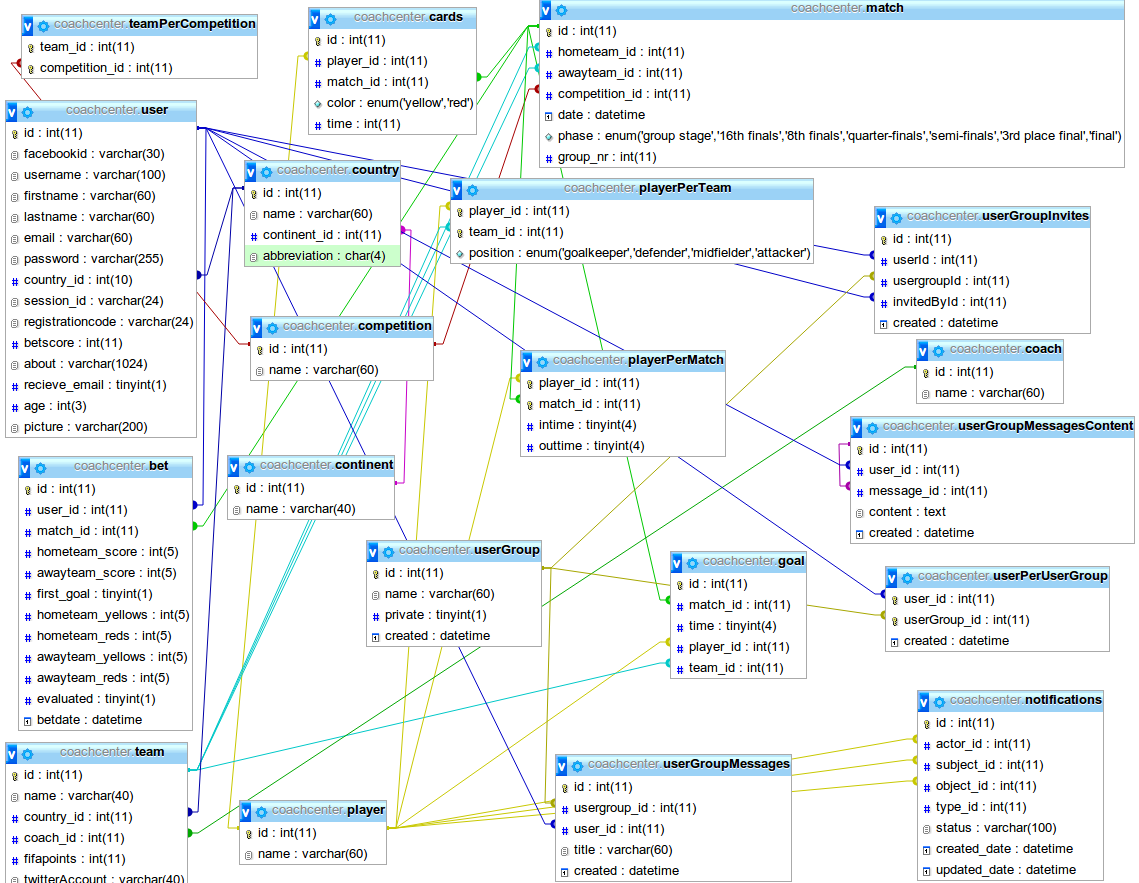
\includegraphics[width=90mm]{ER.png}
\caption{Onze database in ER-model}
\label{overflow}
\end{figure}

\end{document}
